\documentclass[../../../main]{subfiles}
\begin{document}

\section{課題}

\subsection*{問1}
電気伝導率$\sigma$、電気抵抗率$\rho$の定義と単位、その関係は次のとおりである。
電気伝導率$\sigma$は、物質中における電気伝導のしやすさを表す物理量。
単位はSI単位系では、\si{\siemens\per\meter} / \si{\ampere\per\volt\per\meter} / \si{\per\ohm\per\meter}などで表される。
電気抵抗率$\rho$は物質中における電気伝導のしづらさを表す物理量。
単位はSI単位系で、\si{\ohm\meter}で表される。
これら$\sigma$と$\rho$は次の逆数の関係にある。
\begin{equation}
	\sigma = \frac{1}{\rho}
\end{equation}

\subsection*{問2}
次の図\ref{fig:hall-effect}のように、板状または棒状の半導体に対し、
$x$方向に電流$I_x$を流し、$z$方向に磁場$B_z$を印加する。
半導体中を移動するキャリアは、ローレンツ力により、$y-$方向に偏向される。
この偏りによって電場$E_H$が生じ、キャリアが電子の場合$y-$方向、正孔の場合$y+$方向を向く。
このホール電場から受ける力とローレンツ力が釣り合うときが定常状態で、
このときの上面と下面の電位差をホール電圧$V_H$といい、
\begin{align}\label{eq:asg:hall-voltage}
	I_x B_z x & = q (n x y t) \dfrac{V_H}{y} \nonumber \\
	V_H       & = \dfrac{I_x B_z}{q n t}               \\
	          & = R_H \dfrac{I_x B_z}{t}
\end{align}
である。
ただし、$x, y, t$はそれぞれ$x, y, z$方向の半導体の長さ、$q$は電荷、$n$はキャリア数密度である。
また、
\begin{equation}\label{eq:asg:hall-coefficient}
	R_H = \dfrac{1}{q n}
\end{equation}
をホール係数という。

\subsection*{問3}
\ref{eq:asg:hall-coefficient}式より、キャリア数密度は、
\begin{equation}\label{eq:asg:carrier-density}
	n = \dfrac{1}{q R_H}
\end{equation}
とかける。

\subsection*{問4}
移動度$\mu$の単位は\si{\meter\squared\per\volt\per\second}である。

\subsection*{問5}
移動度$\mu$は、
\begin{equation}\label{eq:asg:mobility}
	\sigma = \dfrac{1}{\rho} = q n \mu
\end{equation}
と表され、\ref{eq:asg:carrier-density}式を代入すると、
\begin{equation}\label{eq:asg:mobility-1}
	\mu = \sigma R_H
\end{equation}
と表される。


\begin{figure}
	\centering
	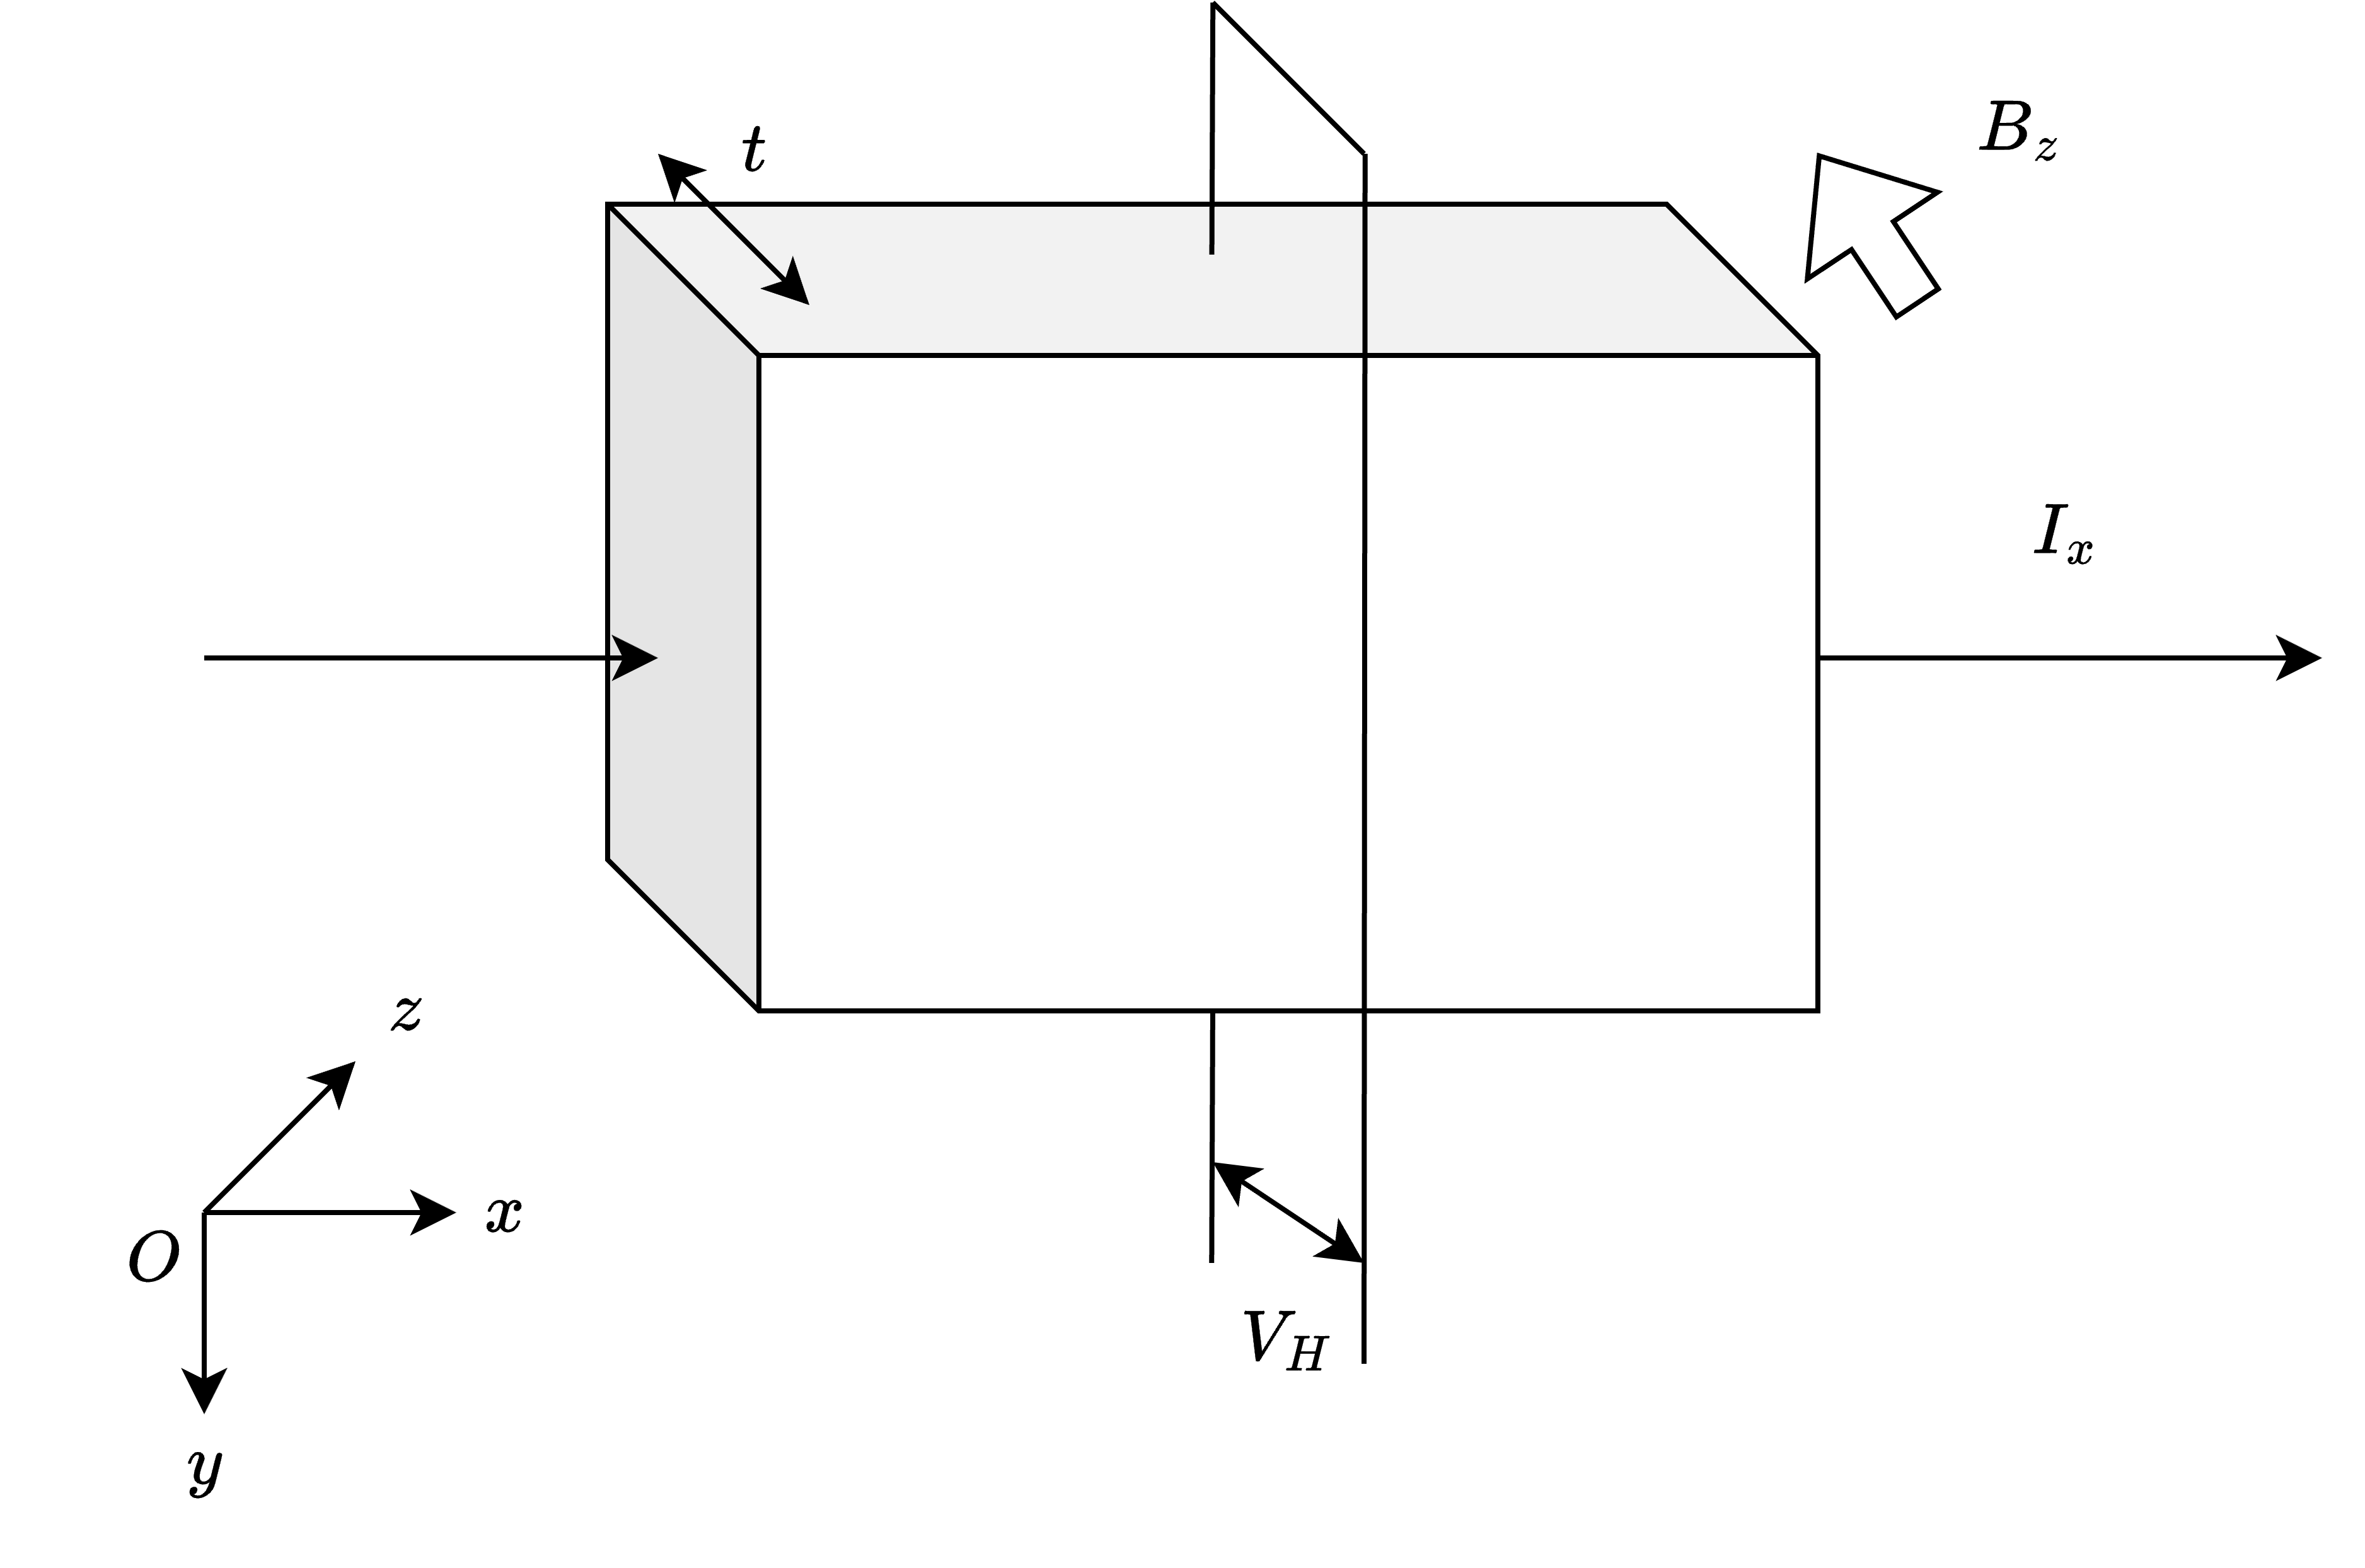
\includegraphics[width=0.8\linewidth]{src/figures/hall/hall.png}
	\caption{ホール効果の実験装置}\label{fig:hall-effect}
\end{figure}



\end{document}
